%% ITU journal paper proposal template for LaTeX
%% Template by: Chiara Debenedetti (chiara.cesira@gmail.com)

%%%== document type ==%%%
\documentclass[10pt,a4paper,twocolumn]{article}
%%%=========%%%

\usepackage{fontspec}
\setmainfont[Ligatures={TeX,Common}]{Cambria}

%%%== packages ==%%%
\usepackage{lineno}
\usepackage{nopageno}
\usepackage{fontspec}
\usepackage{authblk}
\usepackage{graphicx}
\usepackage[explicit]{titlesec}
\usepackage[labelfont=bf,labelsep=endash,font=footnotesize]{caption}
\usepackage{tabu}
\usepackage{xcolor}
\usepackage[hidelinks]{hyperref}
\usepackage[hang]{footmisc}
\usepackage[normalem]{ulem}
\usepackage[top=2.5cm, bottom=2.8cm, left=1.5cm, right=1.5cm]{geometry}
\usepackage{abstract}
\usepackage{mathtools}
\usepackage{amsmath}
\usepackage{amssymb}
\usepackage{balance}
%%%=========%%%

%% Package for creating better tables
\usepackage{multirow}
%%Include standalone files, e.g., tikz figures
\usepackage{pgfplots}
\usepackage{tikz}
\usepackage{standalone}
%Special Tikz markings
\def\checkmark{\tikz\fill[scale=0.4](0,.35) -- (.25,0) -- (1,.7) -- (.25,.15) -- cycle;}
%%Algorithm Design
\usepackage{algorithm}
\usepackage{algpseudocode}

\DeclareMathOperator*{\argmax}{arg\,max}
\DeclareMathOperator*{\argmin}{arg\,min}
\renewcommand{\vec}[1]{\boldsymbol{#1}}
\newcommand{\norm}[1]{\left|\left|#1\right|\right|}

% DEFINING spaces for the neural network:
\def\layersep{2cm}
\def\layersep{2.75cm}

%%%== definitions of new commands/redefinition of existing ones, specifically for this template ==%%%
%\usepackage{unicode-math}
%\setromanfont{Cambria}
%\setmathfont{Cambria}

\makeatletter
\renewcommand\AB@affilsepx{, \protect\Affilfont}
\makeatother

\providecommand{\keywords}[1]{\textbf{Keywords}\ \ \textendash\ \   #1}

\renewcommand{\figurename}{Fig.}

\titleformat{\section}{\large\bfseries}{\thesection.}{1em}{\MakeUppercase{#1}}
\titlespacing*{\section}{0pt}{12pt}{6pt}

\titleformat{\subsection}{\large}{\thesubsection}{1em}{#1}
\titlespacing*{\subsection}{0pt}{12pt}{6pt}

\titleformat{\subsubsection}{\large\itshape}{\thesubsubsection}{1em}{#1}
\titlespacing*{\subsubsection}{0pt}{12pt}{6pt}

\newcommand{\ITUurl}[1]{\textcolor{blue}{\urlstyle{same}\url{#1}}}

\newcommand{\ITUnote}[1]{\begin{small} \ITUpar NOTE: #1 \end{small}}

\setlength{\parindent}{0cm}
\newcommand{\ITUpar}{\vspace{8pt}\par}

\setlength\footnotemargin{0cm} 
\newcommand{\ITUfootnote}[1]{\footnote{#1}}

\renewenvironment{abstract}
               {\list{}{
               \setlength{\rightmargin}{0mm}
               \setlength{\leftmargin}{0mm}
               \vspace{-0.25in}
                \item[\textit{\textbf{\hspace{22pt}Abstract  }}  \textendash]\relax}}
               {\endlist}
\setlength{\columnsep}{1cm}

\setlength{\intextsep}{6pt}
\setlength{\floatsep}{6pt}
\setlength{\textfloatsep}{6pt}

\def\starttable{\vspace{6pt}\begin{table}[ht]\center}
\def\startfigure{\vspace{6pt}\begin{figure}[ht]\center} 

\renewcommand\theequation{\textit{(\arabic{equation})}}
\makeatletter
\def\tagform@#1{\maketag@@@{\ignorespaces#1\unskip\@@italiccorr}}
\makeatother

\setlength{\affilsep}{0em}

\usepackage{caption}
\usepackage{subcaption}

\renewcommand{\Authands}{, }
%%%=========%%%

%%%== TITLE AND AUTHOR DEFINITIONS GO HERE ==%%%
\title{\large{\textbf{\uppercase{Federated Learning for Spatial Reuse Optimization in Future IEEE 802.11 WLANs}}}}

\def\correspondingauthor{\ITUnote{Corresponding author: Francesc Wilhelmi, fwilhelmi@cttc.cat}}

\author[1]{\normalsize{Francesc~Wilhelmi}}
\author[2]{\normalsize{Jernej~Hribar}}
\author[3]{\normalsize{Selim~F.~Yilmaz}}
\author[3]{\normalsize{Emre~Ozfatura}}
\author[3]{\normalsize{Kerem~Ozfatura}}
\author[4]{\normalsize{Ozlem~Yildiz}}
\author[3]{\normalsize{Deniz~G\"{u}nd\"{u}z}}
\author[5]{\normalsize{Hao~Chen}}  
\author[5]{\normalsize{Xiaoying~Ye}}  
\author[5]{\normalsize{Lizhao~You}}
\author[5]{\normalsize{Yulin~Shao}}
\author[1]{\normalsize{Paolo~Dini}}
\author[6]{\normalsize{Boris~Bellalta}}

\affil[1]{\normalsize{CTTC (Spain)}}
\affil[2]{\normalsize{CONNECT~Centre, Trinity~College~Dublin (Ireland)}}
\affil[3]{\normalsize{King's~College~London (United Kingdom)}}
\affil[4]{\normalsize{New~York~University (USA)}}
\affil[5]{\normalsize{Xiamen~University (China)}}
\affil[6]{\normalsize{Universitat~Pompeu~Fabra (Spain)}}

\date{\vspace{-12pt}{\small NOTE: Corresponding author: Francesc Wilhelmi, francesc.wilhelmi@cttc.cat} \\  \endgraf\rule{\textwidth}{1pt}}

%\date{\vspace{-12pt}\endgraf\rule{\textwidth}{1pt}}

%%%=========%%%


%%%== start of the actual document ==%%%
\begin{document}

%\linenumbers %% this should be commented out if line numbers in the text are not wanted

%%= title and abstract =%%
\twocolumn[

\begin{@twocolumnfalse}
\maketitle

%%= abstract text � SUBSTITUTE HERE! =%%
\begin{abstract}
\textit{As wireless standards evolve, more complex functionalities are introduced to address the increasing requirements in terms of throughput, latency, security, and efficiency. To unleash the potential of such new features, artificial intelligence (AI) and machine learning (ML) are currently being exploited for deriving models and protocols from data, rather than by hand-programming. In this paper, we explore the feasibility of applying ML in next-generation IEEE Wireless Local Area Networks (WLANs). More specifically, we focus on the IEEE 802.11ax Spatial Reuse (SR) problem and predict its performance through Federated Learning (FL) models. The set of FL solutions overviewed in this work is part of the 2021 International Telecommunication Union (ITU) AI for 5G Challenge.}
\end{abstract}
%%======%%
\ITUpar
%%= keywords =%%
\keywords{Federated learning, IEEE 802.11ax, ITU Challenge 2021, machine learning, network simulator, spatial reuse}
%%======%%

%\ITUnote{Title, abstract and keywords must be identical to the ones submitted electronically in EDAS \textendash\ Editor's Assistant. Use the command \texttt{\textbackslash ITUnote} to achieve the appropriate formatting.}
\ITUpar
\ITUpar

\end{@twocolumnfalse}
]

% the results obtained correspond to the output of the 2021 International Telecommunication Union (ITU) AI for 5G Challenge.

%%= start of sectioning � MODIFY EACH TITLE AND LABEL AS YOU PLEASE =%%
\section{Introduction} 
\label{sec:intro}

Wireless networks are evolving towards Artificial Intelligence (AI) / Machine Learning (ML)-driven systems able to address the overwhelming requirements of future mobile communications~\cite{morocho2019machine,akhtar2020shift}, namely the fifth generation (5G) and Beyond 5G (B5G). The application of ML for networking can be found at different communication layers and parts of a network, e.g., network management to drive the self-organizing networks (SON) paradigm~\cite{klaine2017survey}, optimization of the Medium Access Control (MAC) layer in decentralized channel access~\cite{bkassiny2012survey}, or AI-native physical communication protocols~\cite{oshea2017introduction,hoydis2021toward}. The fact is that AI/ML can leverage the vast amount of network and user data to generate new knowledge that allows improving the network performance and, hence, making progress in the development of novel network applications (e.g., virtual reality).\ITUpar

Nevertheless, the use of ML in communications also raises concerns of different nature. First, ML-based solutions typically require a lot of energy for training complex models (e.g., neural networks) and high bandwidth for exchanging training data, which typically needs to be centralized to a single point. Moreover, the massive usage of networking data for ML may threaten security and users' privacy. The privacy issue may be exacerbated in decentralized networks such as IEEE 802.11 Wireless Local Area Networks (WLANs), whereby the lack of a central network manager may make inter-WLAN interactions unreliable.\ITUpar 

To address some of the challenges posed by traditional ML training, Federated Learning (FL) optimization was introduced in~\cite{federated1} as a distributed training paradigm that allows keeping the data at its source. Since then, a significant number of FL applications have flourished in different fields, such as medicine~\cite{federated2}, autonomous driving~\cite{federated3}, UAV-based wireless networks~\cite{federated4}. FL has become a suitable paradigm to foster collaboration among different parties interested in solving a common problem. Under the management of a central server (typically, a neutral entity), FL participants contribute to building a general ML model, each one using local data, by sharing model weights, rather than raw training data.\ITUpar

In this paper, we study the application of FL models to the IEEE 802.11 Spatial Reuse (SR) problem, which aims to enhance spectral efficiency by adjusting the devices' carrier sense area to increase the number of concurrent transmissions in overlapping deployments. IEEE WLANs are called to be an important part of the B5G ecosystem, as it represents a cost-effective solution for the access network. In particular, we overview the output of the problem statement entitled \textit{``ITU-ML5G-PS-004: Federated Learning for Spatial Reuse in a multi-BSS (Basic Service Set) scenario''}, which was part of the 2021 International Telecommunication Union (ITU) AI for 5G Challenge~\cite{bib2}.\footnote{The ITU AI/ML challenge is a global competition that gathers professionals, researchers, practitioners, and students from all around the globe to solve relevant problems on ML for communications.} In the proposed problem statement, a data set with simulated IEEE 802.11ax (11ax) measurements was provided to develop FL solutions able to predict, and therefore optimize, the performance of next-generation, crowded Wi-Fi deployments applying SR. The usage of simulated data for enriching training data sets is another relevant topic for enabling ML in communications~\cite{wilhelmi2021usage}.\ITUpar

The main contributions of this paper are as follows:
\begin{itemize}
	\item We overview the SR technology for both 11ax and future amendments and propose the usage of FL to address it.
	\item We provide a data set with 11ax SR measurements for next-generation WLANs. The data set is open and can be accessed at~\cite{dataset}. 
	\item We overview the set of FL solutions proposed by the participants of the 2021 ITU AI for 5G Challenge. Table~\ref{tab:tab0} briefly summarizes the proposed models, as well as the main motivation behind them.
\end{itemize}\ITUpar

\starttable
\caption{Summary of the ML models proposed by the participants of the challenge \textcolor{red}{(to be done)}.}\label{tab:tab0} 
\begin{small}
	\resizebox{\columnwidth}{!}{%
	\begin{tabular}{|c|c|c|c|}
		\hline
		\textbf{Team} & \textbf{Proposed Model} & \multicolumn{1}{c|}{\textbf{Motivation}} & \textbf{Ref.} \\ \hline
		FederationS & \begin{tabular}[c]{@{}l@{}}DNN with two\\parallel branches\end{tabular} & \begin{tabular}[c]{@{}l@{}}Exploit relationships among\\training features\end{tabular} & \cite{federations2021repository} \\ \hline
		\begin{tabular}[c]{@{}c@{}}FedIPC\end{tabular} & \begin{tabular}[c]{@{}c@{}}NN with a Multi-Output \\Regression Objective\end{tabular} & \begin{tabular}[c]{@{}l@{}}Take advantage of knowledge\\on wireless operation\end{tabular} &  \cite{wirelessai2021repository}\\ \hline
		\begin{tabular}[c]{@{}c@{}}WirelessAI\end{tabular} & \begin{tabular}[c]{@{}c@{}}\end{tabular} & \begin{tabular}[c]{@{}l@{}}\end{tabular} & \cite{fedipc2021repository} \\ \hline
	\end{tabular}
	}
\end{small}
\end{table}

The rest of the paper is structured as follows. Section~\ref{section:spatial_reuse} introduces the SR problem in 11ax and future WLANs. Section~\ref{section:federated_learning} provides some basics on FL are provided, with especial emphasis on its application in networking applications. Section~\ref{section:dataset} overviews the provided SR data set for training ML models. The solutions proposed by the challenge participants are described in detail in Section~\ref{section:solutions} and evaluated in Section~\ref{section:performance}. Section~\ref{section:conclusions} concludes the paper with some remarks and future directions.

\section{Spatial Reuse in 802.11ax WLANs: overview and research gaps}
\label{section:spatial_reuse}

IEEE 802.11 technology, commonly known as Wi-Fi, is one of the most popular solutions for the access network due to its easiness of deployment and low cost (it operates on unlicensed bands). However, its fundamental operation is based on Carrier Sense Multiple Access (CSMA), which is well known to degrade performance when dealing with a high number of concurrent users~\cite{ziouva2002csma}. To address the issues raised by network density and meet the increasingly strict requirements posed by next-generation applications (e.g. Virtual Reality), 802.11 amendments introduce novel functionalities and protocol enhancements. For instance, standards 802.11n (2009) and 802.11ac (2013) provided High Throughput (HT) and Very High Throughput (VHT) devices by including, for instance, the application Channel Bonding (CB), whereby basic channels could be aggregated to increase the capacity of a single transmission.\ITUpar

	As for the SR operation~\cite{bib9}, it was recently introduced by the IEEE 802.11ax (2021) standard~\cite{bellalta2016ieee} to increase the number of parallel transmissions in Overlapping Basic Service Sets (OBSS). Among other features like Orthogonal Frequency Division Multiple Access (OFDMA), or Downlink/Uplink Multi-User Multiple Input-Multiple-Output (MU-MIMO), SR aims at enhancing performance and efficiency. To do so, it provides two different operational modes:
\begin{enumerate}
	\item OBSS Packet Detect-based SR (OBSS/PD-based SR).
	\item Parametrized Spatial Reuse (PSR).
\end{enumerate}

The main difference between the two mechanisms lies in the way SR Transmission Opportunities (TXOPs) are detected by devices implementing them. While OBSS/PD-based SR operates in the downlink, PSR is thought for the uplink. In what follows, we focus on OBSS/PD, which has gained more interest and has been considered to evolve in future amendments like the IEEE 802.11be (11be)~\cite{lopez2019ieee}. A comprehensive overview of these two mechanisms can be found in~\cite{bib9}.\ITUpar

In essence, OBSS/PD-based SR allows devices to transmit in parallel with others that gained the channel access beforehand. To do so, a new OBSS/PD threshold is defined to be applied when an incoming detected transmission marks the radio channel as busy through Clear Channel Assessment (CCA) operation. The CCA allows overlapping devices to share a common channel and is triggered when identifying the preamble of a Wi-Fi transmission. Provided that the OBSS/PD threshold allows initiating a new SR transmission, a transmit power limitation must be applied so that the additional generated interference does not affect the original transmission.\ITUpar

\startfigure
\begin{subfigure}[b]{\linewidth}
	\centering
	\includegraphics[width=.75\textwidth]{img/obsspd_1}
	\caption{}
	\label{fig:obsspd_1}
\end{subfigure}
\begin{subfigure}[b]{.75\linewidth}
	\centering
	\includegraphics[width=\textwidth]{img/obsspd_2}
	\caption{}
	\label{fig:obsspd_2}
\end{subfigure}
\caption{IEEE 802.11ax OBSS/PD-based SR operation: (a) signal reception areas, (b) diagram with packets exchange.}\label{fig:sr_operation} 
\end{figure}

The OBSS/PD SR operation is illustrated in Fig.~\ref{fig:sr_operation} for two overlapping APs. As shown in Fig.~\ref{fig:obsspd_1}, Access Point A (AP$_\text{A}$) detects the signals from all the considered devices (represented by the red area), including AP$_\text{B}$ and Station B (STA$_\text{B}$), which belong to a different BSS. In particular, AP$_\text{B}$ is inside the carrier sense area of AP$_\text{B}$ (represented by the gray area), so they both must contend for the channel whenever the other starts a transmission (e.g., to its associated STAs). Nevertheless, thanks to the OBSS/PD-based SR operation, AP$_\text{A}$ can ignore AP$_\text{B}$'s transmissions when applying the OBSS/PD threshold (represented by the green area). At the packet level (shown in Fig.~\ref{fig:obsspd_2}), AP$_\text{A}$ starts decoding the preamble of new transmission from AP$_\text{B}$, which has initially gained the access to the medium using Carrier Sense Multiple Access with Collision Avoidance (CSMA/CA). From the preamble reception, AP$_\text{A}$ determines that the channel is busy at the MAC layer due to the CCA operation. But, using the SR mechanism, AP$_\text{A}$ identifies an SR TXOP because the incoming signal is below the OBSS/PD threshold. Hence, AP$_\text{A}$ can initiate a transmission before AP$_\text{B}$ leaves the channel, provided that a transmit power restriction is applied (see Eq.~\eqref{eq:tx_power_limit}) for the sake of not affecting AP$_\text{B}$'s transmission.

\begin{equation}
	\scriptsize
	\text{TX\_PWR}_\text{max} = \text{TX\_PWR}_\text{ref} - (\text{OBSS/PD} - \text{OBSS/PD}_\text{min}),	\label{eq:tx_power_limit}
\end{equation}

where $\text{TX\_PWR}_\text{ref}$ is the transmit power reference (set to 21 dBm or 25 dBm, depending on the device's antenna capabilities), $\text{OBSS/PD}$ is the selected OBSS/PD threshold for detecting SR TXOPs, and $\text{OBSS/PD}_\text{min}$ is the minimum OBSS/PD threshold (fixed to -82 dBm).\ITUpar

While SR promises to enhance spectral efficiency in dense OBSS deployments, its actual performance is hindered by the proper election of the OBSS/PD threshold, which may not be trivial due to the complex inter-device interactions in a WLAN. The fact is that the OBSS/PD-based SR operation is a decentralized mechanism that only considers the interactions between principal transmitters (i.e., devices gaining access to the channel for transmitting), but does not account for the interference at the recipients of such transmissions nor the impact of uplink control frames (e.g., acknowledgment packets). Since the standard does not provide any method for selecting the proper OBSS/PD threshold, there is an imperative need for finding mechanisms able to leverage the SR operation.\ITUpar

In this regard, ML may be of great utility and help capturing the complex interactions among IEEE 802.11 devices applying SR. Most of the literature in this subject has so far focused on Reinforcement Learning (RL) and online learning techniques, whereby agents attempt to learn the best OBSS/PD configuration sequentially. In~\cite{wilhelmi2019collaborative, wilhelmi2019potential}, the authors modeled the decentralized SR problem through Multi-Armed Bandits (MAB), an online learning framework whereby agents attempt to address the exploration-exploitation trade-off. While~\cite{wilhelmi2019collaborative} studied the problem by using selfish rewards in a competitive environment,~\cite{wilhelmi2019potential} introduced the usage of shared rewards for the sake of maximizing fairness. Other RL-based approaches can be found in~\cite{bardou2021improving} and~\cite{yin2019learning}.\ITUpar

The online learning paradigm turns out to be a cost-effective solution to the decentralized SR problem, due to its ability for solving complex partial information problems. In addition, WLANs typically experience a high variability both in terms of devices' mobility and activation/deactivation, so past learned information may become easily outdated. However, as shown in~\cite{wilhelmi2019potential}, online learning may have some pitfalls when applied to dense WLANs, mainly raised by the high action-decision space, the non-stationarity of agents reward in competitive settings, or the complexity of finding a proper shared reward, able to maximize the overall network performance.\ITUpar

For those reasons, in this paper, we focus on the suitability of supervised learning methods, mostly based on Deep Learning (DL), for the SR problem in WLANs. To the best of our knowledge, this topic has been barely studied before. For instance,~\cite{jamil2016novel} proposed a centralized DL-based method to jointly select the transmission power and the physical carrier sensing, but out of the context of the 11ax SR operation. Furthermore, DL was applied in~\cite{soto2021atari} to address a similar problem in dense WLANs (channel bonding).\footnote{This and other DL solutions for the dynamic channel bonding problem in IEEE 802.11ax WLANs were overviewed in~\cite{wilhelmi2021machine}.}  For further details on Wi-FI optimization through ML, we refer the interested reader to the comprehensive survey in~\cite{szott2021wifi}.\ITUpar

Notice, as well, that the overviewed works on DL consider centralized approaches, which require data to be gathered at a single point for training a typically static model that is used homogeneously across all the AI-enabled devices. Nevertheless, in practice, some deployments (e.g., residential WLANs) may have limitations in terms of computation, storage, or communication capabilities (for instance, low-throughput connections, intermittent availability). Moreover, separate WLAN deployments can be substantially different, thus requiring specialized models (rather than general ones). To address the issues of centralized learning on heterogeneous deployments, we focus on the FL paradigm, introduced in the next section.\ITUpar

\section{An Introduction to Federated Learning for Networking}
\label{section:federated_learning}

The FL optimization paradigm was first introduced in~\cite{konevcny2016federated} to address some critical issues of traditional centralized ML mechanisms. In FL, training is done at end devices (or clients), which do not share their training data with others. Instead, ML model updates are provided and aggregated under the management of a typically central server. By removing the procedures related to data exchanging, FL decreases the communication overhead in ML and enhances user privacy and security. Moreover, FL is an appealing solution for dealing with heterogeneous sets of clients, thus allowing to create specialized models according to clients' characteristics. With that, FL has the potential of revolutionizing ML implementations, bringing them closer to practical applications and use cases. Some examples can be found medicine~\cite{nguyen2021federated2}, finance~\cite{long2020federated}, industry 4.0~\cite{que2020blockchain}, or telecommunications~\cite{lim2020federated}.\ITUpar

In the telecommunications realm, novel ML for communications solutions lead to handling a vast amount of data. These kinds of resource-demanding applications may threaten the stability of the network on the one hand and may experience low performance due to the communication bottleneck on the other hand. FL can potentially alleviate some of these issues by reducing the overheads generated by the ML operation while providing good performance. Furthermore, the usage of FL contributes to enhancing privacy, which is a critical issue in communications. FL applications in communications~\cite{yang2021federated} include autonomous driving~\cite{li2021privacy}, unmanned aerial vehicle (UAV)-based wireless networks~\cite{brik2020federated}, edge computing~\cite{wang2019inedge}, or Internet-of-Things (IoT) intelligence~\cite{khan2021federated}.\ITUpar

The way FL operates is as follows (see Fig.~\ref{fig:federated_optimization}): 
\begin{enumerate}
	\item A set of $\mathcal{K}=\{1,2,...,K\}$ clients download a initial model, typically provided by the server.
	\item Clients perform training using their local data points $\{x_k,y_k\}$ (with size $N_k$) and update the model weights accordingly, denoted by $w_k\in \mathbb{R}^d$. At this point, it is important to highlight the federated averaging (FedAvg) method~\cite{mcmahan2017communication}, which is based on stochastic gradient descent (SGD) optimization and performs well for non-convex problems. 
	\item The server pulls data from clients (a subset of clients may be selected in each FL round for the sake of performance)  and orchestrates weight aggregation to generate a global model $w\in \mathbb{R}^d$.
	\item The global model $w$ is sent back to clients, so that a new training iteration $t\in T$ is done.
	\item The above steps are repeated until convergence, i.e., until a time horizon is completed or until certain accuracy goals are met. 
\end{enumerate} 

\startfigure
\includegraphics[width=\columnwidth]{img/federated_optimization}
\caption{FL optimization in different WLAN contexts.}\label{fig:federated_optimization} 
\end{figure}

Using FedAvg, clients perform several batch updates using local data to update model parameters. Unlike for classical Federated Stochastic Gradient Descent (FedSGD), where gradients are exchanged, FedAvg considers sharing model weights (e.g., the parameters of a neural network). By applying multiple rounds of training, FL seeks to minimize a global finite-sum cost function $l(w)$ by optimizing the global model parameters $w$:
\begin{equation}
	\min_{w \in \mathbb{R}^d} l(w) = \min_{w\in \mathbb{R}^d} \sum_{k=1}^{K} \frac{N_k}{N} l_k(w,x_k,y_k),
	\label{eq:fl_loss_goal}
\end{equation}
where $l_k(w,x_k,y_k)$ is the loss experienced by client $k$ when using the global model $w$ on its local data, and $N$ is the total size of the distributed data set, i.e., $N = \sum_{\forall k \in \mathcal{K}} N_k$.\ITUpar

To compute local updates, clients run $E$ epochs of SGD based on the target local loss function $l_k$ and the batch size $B$ applied to local data $\{x_k,y_k\}$. Being $\eta$ the learning rate, local updates are thus given by:
\begin{equation}
	w_k^{t+1} \leftarrow w_k^t - \eta \nabla l_k(w^t,x_k,y_k)
	\label{eq:fl_local_update}
\end{equation}

Finally, being $\eta$ the learning rate, the server aggregates clients' weights based on the importance $\gamma_k$ assigned to each client which may be set according to local data set lengths (as indicated in Eq.~\eqref{eq:fl_loss_goal}):
\begin{equation}
	w^{t+1} = \sum_{k=1}^{K} \gamma_k w_k^t  
	\label{eq:fl_aggregation}
\end{equation}
 
Beyond FedAvg, other optimization mechanisms have been proposed to improve on convergence and efficiency aspects~\cite{reddi2020adaptive}. For further details on FL, we refer the interested reader to the works in~\cite{zhang2021survey, li2020federated}.\ITUpar

\section{Open simulated data set on IEEE 802.11ax SR}
\label{section:dataset}

Supervised ML methods typically require a significant amount of high-quality data to perform well. Training data is usually obtained either from network activity~\cite{turkcelldataset} or from measurement campaigns~\cite{barrachina2021wifi}. However, obtaining real traces from networks can be challenging due to proprietary limitations (data owners are reluctant to share their assets), data privacy issues (most network data is generated by final users), or difficulties in obtaining data from a rich set of situations (anomalies are hard to reproduce and identify). In this sense, the usage of synthetic data sets for model training is gaining attention~\cite{wilhelmi2021usage}. Such data sets can be obtained, for instance, from network simulators (e.g., ns-3, OMNET++, OPNET). Simulators are a cost-effective solution for generating comprehensive data sets. Some prominent examples of synthetic data sets oriented to ML training can be found in~\cite{suarez2021graph, dataset2020}.\ITUpar

As for the provided data set on 11ax SR~\cite{dataset}, it has been generated with Komondor~\cite{bib8}, an open-source IEEE 802.11ax-oriented simulator that includes features like channel bonding or SR. Komondor does not implement the targeted functionalities, but its execution is also lightweight, thus allowing for generating large data sets corresponding to massive WLAN deployments.\ITUpar

The data set contains both training and test files, which include the results obtained from several simulated random deployments applying 11ax SR (see the example random deployment in Fig.~\ref{fig:simulation_scenario}). More specifically, a set of three baseline scenarios was considered to represent different types of deployments. Considering the features in each type of scenario (e.g., maximum number of STAs per BSS, minimum distance between APs), 1,000 random deployments of each type were generated for training. Each simulated deployment corresponds to a context $k\in \mathbb{K}$, where the BSS of interest (namely, BSS$_\text{A}$) is used as a client for FL optimization. To enrich contexts with data, each BSS includes information for each possible OBSS/PD configuration $\tau$ (i.e., from -82 dBm to -62 dBm with 1 dBm precision). Finally, for the test data set, 1,000 more deployments were simulated using more relaxed constraints. In this case, a single random OBSS/PD configuration was selected in each deployment. Table~\ref{tab:tab1} provides an overview of the entire data set.\ITUpar

\startfigure
\includegraphics[width=.8\columnwidth]{img/simulation_scenario}
\caption{Example of a simulated WLAN deployment.}\label{fig:simulation_scenario} 
\end{figure}

\starttable
	\caption{Summary of the scenarios of the data set.}\label{tab:tab1} 
	\resizebox{\linewidth}{!}{\begin{tabular}{|c|c|c|c|c|c|}
			\hline
			& \textbf{Sce id} & \textbf{Num. APs} & \textbf{Num. STAs} & \textbf{d\_min(APs)} & \textbf{\begin{tabular}[c]{@{}c@{}}Context \\ variations\end{tabular}} \\ \hline
			\multirow{3}{*}{\textbf{Training}} & training1 & \multirow{4}{*}{2-6} & 1 & 10 m & None \\ \cline{2-2} \cline{4-6} 
			& training2 &  & 1-4 & 10 m & None \\ \cline{2-2} \cline{4-6} 
			& training3 &  & 1-4 & None & \begin{tabular}[c]{@{}c@{}}Up to 20 \\ locations\end{tabular} \\ \cline{1-2} \cline{4-6} 
			\textbf{Test} & test &  & 2-4 & None & None \\ \hline
	\end{tabular}}
\end{table}

Training scenario \textit{training1} considers BSSs with only one STA, which is useful to minimize the impact of uplink transmissions, thus allowing to focus on inter-AP interactions only. In contrast, scenarios \textit{training2} and \textit{training3} consider up to 4 STAs per AP, which contribute generating more traffic in the uplink. As for the minimum distance between APs (d$_\text{min}$), it is set to 10~m in scenarios \textit{training1} and \textit{training2}, whereas the rest have no limitation. Furthermore, contexts in scenario \textit{training3} contain richer datasets by simulating variations of the same deployments using different STA locations. \ITUpar

The information included in simulated files is divided into features and label. Concerning features for training, we find the following key elements:
\begin{enumerate}
	\item \textbf{Type of node:} indicates whether the node is an AP or an STA.
	\item \textbf{BSS id:} identifier of the BSS to which the node belongs.
	\item \textbf{Node location:} \{x,y,z\} position of nodes in the map.
	\item \textbf{Primary channel:} main frequency channel used for transmitting and for carrier sensing.
	\item \textbf{Transmit power:} default transmit power used for transmitting frames.
	\item \textbf{OBSS/PD threshold:} sensitivity used within the OBSS/PD-based SR operation.
	\item \textbf{Received Signal Strength Indicator (RSSI):} average signal quality experienced by STAs during reception phases.
	\item \textbf{Inter-BSS interference:} average power sensed from devices belonging to other BSSs.
	\item \textbf{Signal-to-Interference-plus-Noise Ratio (SINR):} average SINR experienced by STAs when receiving data from their AP.
\end{enumerate}

It is worth noting that most of the extracted information is typically obtained on a continuous basis in a real system. Indeed, the RSSI, SINR and throughput measurements can be reported periodically by STAs. Interference powers can be measured during the listen-before-transmit (LBT) phase at the AP, employing multi-antenna processing techniques to separate the different interfering sources. In addition, Time-of-Arrival (TOA) ranging techniques can determine the distance between STAs and APs.\ITUpar

As for the label, we provide the throughput $\gamma_{k,j}$ obtained by each STA $j$ in context $k$ during the simulation. Predicting the throughput is the goal of the implemented FL solutions described in the next section. Notice, as well, that other Key Performance Indicators (KPIs) such as the average delay or the number of SR TXOPs could have been considered.\ITUpar

%\startfigure
\begin{figure*}[t!]
	\centering
	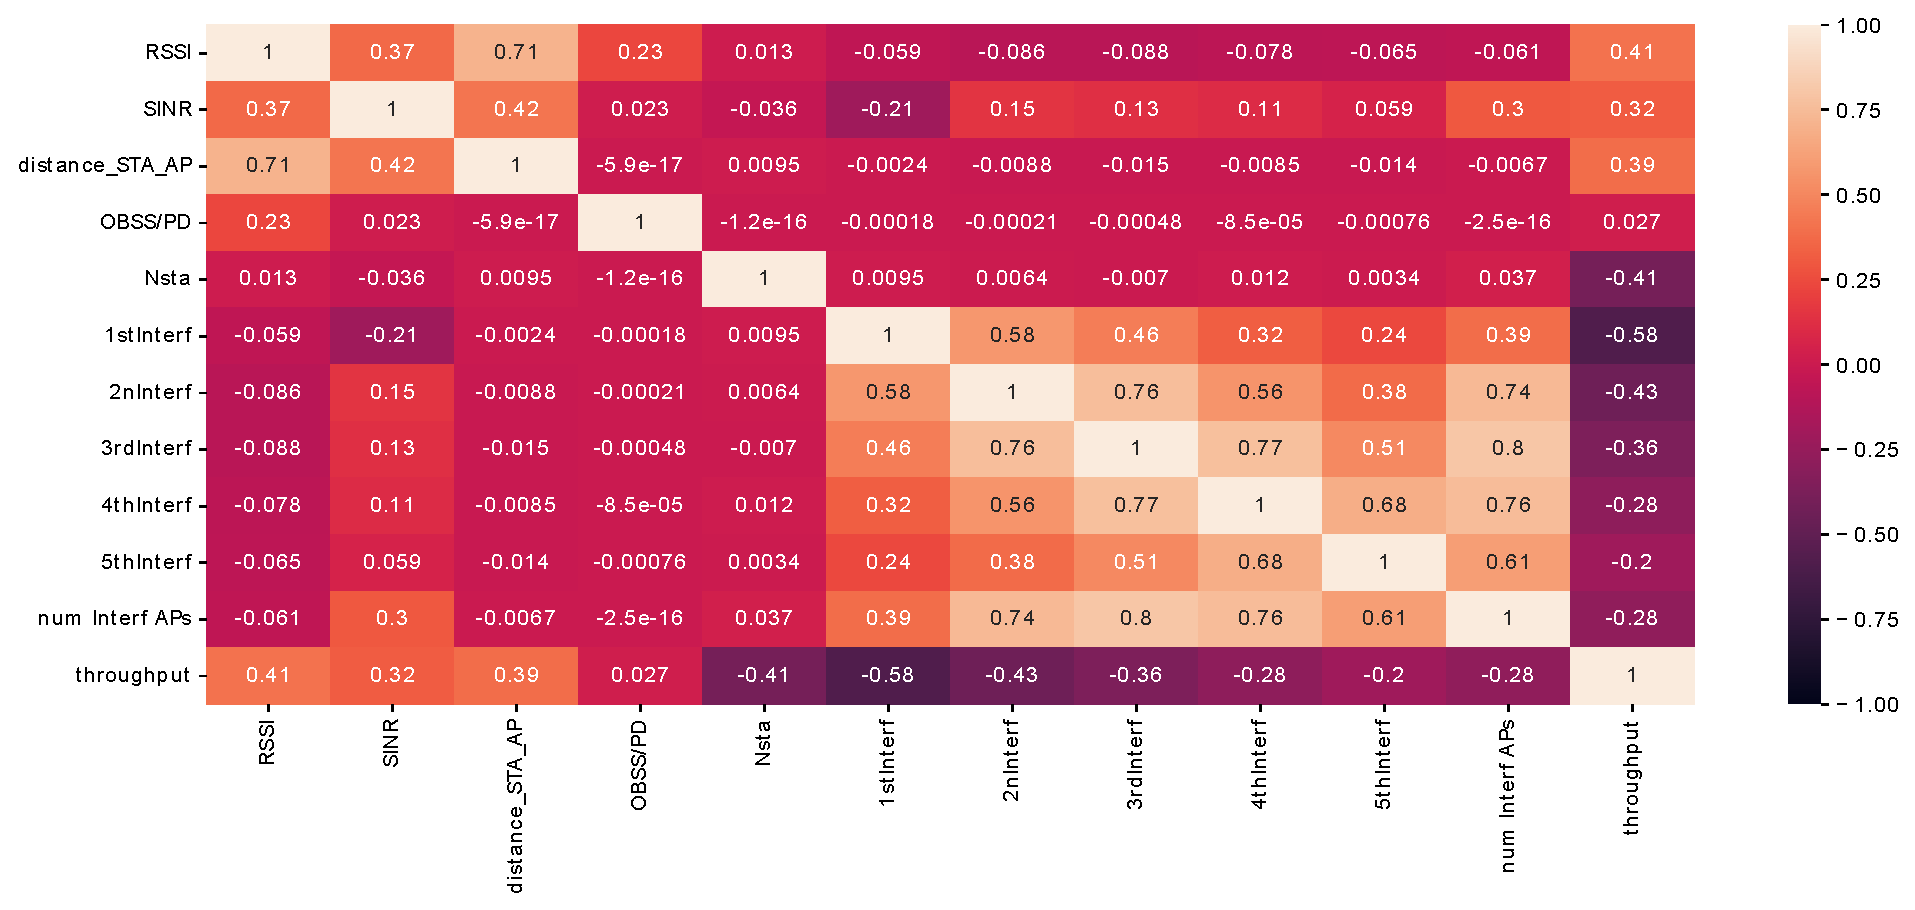
\includegraphics[width=.8\linewidth]{img/Correlation_heatmap_r.eps}
	\caption{Correlation between different input and output variables of the dataset.}
	\label{fig:Correlation heatmap}
\end{figure*}

To conclude this section, we show the correlation matrix between input and output variables in Fig.~\ref{fig:Correlation heatmap}, which is later used as a motivation for some of the proposed ML solutions. Correlation values close to $0$ indicate a lack of relations and structure between the data corresponding to these variables, while correlation values close to $-1$ and $+1$ indicate a perfect negative and positive correlation between variables, respectively.

\startfigure
\centering
\includegraphics[width=.85\columnwidth]{img/hist_features}
\caption{Histogram features.}
\label{fig:hist_features}
\end{figure} 

\section{Federated Learning Solutions for Throughput Prediction}
\label{section:solutions}

In this section, we describe the solutions proposed by the participants of the 2021 ITU AI for 5G Challenge: \textit{FederationS}, \textit{FedIPC}, and \textit{WirelessAI}.

\subsection{FederationS}

%\subsubsection{FederationS' data pre-processing}
%\label{Sec:preprocessing_feds}

Our solution is designed in three stages. In the first stage, we analyze and pre-process available datasets. In the second stage, using gained insights from the data analysis, we define a DNN model running in each client. In the final stage, we describe the proposed FL algorithm. \ITUpar

In the data analysis stage, we consider scenarios \textit{training2} and \textit{training3}, containing $2000$ different IEEE 802.11ax deployments (see Table~\ref{tab:tab1} for further details). We extract several features available in the simulator’s output files from these scenarios, namely the OBSS/PD configuration, the RSSI, the interference at the reference AP from other APs, the SINR, and the throughput of each STA. We also obtain additional information using available data in the simulator’s input files. In particular, we extract the coordinates of APs and STAs to compute the Euclidean distances among them. In addition, we obtain the number of STA served by the reference AP and the number of interfering APs.\ITUpar

To obtain the final dataset to be used to train our model, we pre-process the data through different steps. First, we clean the input and output data parsed from the simulator files removing all non-numerical values from the dataset. Then, we arrange the data of each STA to form 1-D vectors with $11$ numerical entries used as the input of the model and containing all measurements and system parameters. Conversely, we define the STA throughput as the target variable and output of the model. To note that the features present entirely different ranges between maximum and minimum values and are expressed with different units of measurements, e.g. dBm for RSSI and interference power, dB for SINR, and meters for distances. To balance each feature's contribution to the overall model predictions, we re-scale the features with the Min-Max normalization method that transforms all features' in the range $[0,1]$. Finally, when input data are missing, like when the number of interfering AP reported is less than the minimum recorded according to our system settings, we assign those values with $0$s. The activation function that we will explain later is chosen to keep neurons inactive when $0$s are present at the input.\ITUpar

%\subsubsection{DNN Model Design}
%\label{Sec:Centralised Solution}

%\subsubsection{FederationS' proposed solution}

To decide the ML method to be used, we make the following two main observations from the correlation analysis done in Fig.~\ref{fig:Correlation heatmap}:
\begin{enumerate}
	\item Most features show a strong positive or negative correlation with the output variable (throughput). As expected, only the OBSS/PD feature does not directly affect the throughput. Otherwise, the problem would be trivial to model. Indeed, the OBSS/PD value is correlated to the RSSI, which affects SINR and throughput variables, showing that relationships between input and output values of the system are not straightforward to characterize with domain-based models. This justifies the adoption of DNN, which are extensively used for their capabilities to model nonlinear relationships. 
	%
	\item Two regions depicted with lighter colors at the top left and at the bottom right of the correlation matrix identify two groups of features that show a strong positive correlation between input variables. Thus, in the DNN architecture design, these inputs of the model need to be fully connected. In contrast, the two regions at the top right and bottom left are characterized by elements with close to zero correlation values, meaning that the relationship between features is weak. Therefore, these connections are expected to bring a low contribution to the predictions and can be dropped in the DNN architecture design. 
\end{enumerate}

Based on this, in the following design stage, we model DNN architecture as represented in Fig.~\ref{fig:DNN model}. First, we split the DNN model into two parallel branches. The inputs of the first branch are the features constituting the first block, i.e. RSSI, SINR, distance STA-AP, and OBSS-PD threshold. At the same time, features like the number of STA, the power received from interfering AP, and the number of interfering AP form the second block of features and are used as input of the second branch. The input layers are followed by two hidden layers defined for each branch separately. We use a concatenation layer to merge the output of these two branches. The result of the concatenation is then used as input of two additional hidden layers, which are connected to the output layer of the model. We adopt the hyperbolic tangent (\emph{tanh}) activation function to provide positive and negative outputs and keep neurons inactive when the inputs are $0$s. Finally, we add dropout layers after each layer before the output layer to reduce overfitting.\ITUpar

\startfigure
\centering
\includestandalone[width=\linewidth]{tikz_figures/ann_small}
\caption{Visualization of FederationS' DNN structure.}
\label{fig:DNN model}
%\vspace{-10pt}
\end{figure}

As for the FL solution, it is based on the implementation outlined in~\cite{federated_repo}. In addition, our approach combines the trained weights in a novel way, which is designed specifically for this challenge and is based on the data acquired in each context. In particular, our proposed FL solution follows the steps described in Algorithm~\ref{alg:fed}.\ITUpar

\begin{algorithm}[ht!]
	\caption{FederationS solution.}
	\begin{algorithmic}[1]
		\State Initialize set $\mathbb{K}$, i.e., init $K$ contexts with data samples
		\State From $\mathbb{K}$, select $N_{eval}$ to create $\mathbb{K}_{val}$
		\State Create a new set of contexts $\mathbb{K}_{tr} =  \mathbb{K} \cap \mathbb{K}_{val}$
		\State Server initializes model parameters $\theta^0$ and $W^0$
		\State The server transmits $\theta_k^0, w_k^0$ to $k$-th contexts
		\For{communication epoch $t=1,2,...,T$}
		\State Randomly select $N_{tr}$ contexts from $\mathbb{K}_{tr}$ to get $\mathbb{K}_{ep}$
		\For{$i$-th context in $\mathbb{K}_{ep}$}
		%\State The $i$-th context updates the model using %Adam Optimiser and MSE loss
		\State Split samples in $\beta$ ($\frac{n_i}{B}$ batches of size $B$)
		\State Where $n_i$ is the number of data samples 
		\For{batch $b$ in $\beta$}
		\State  $\theta_i^t, w_i^t \leftarrow \theta_i^{t-1}, w_i^{t-1} - \eta \nabla l(\theta_i^{t-1}, w_i^{t-1};b)$
		\EndFor
		\State Determine weight $\alpha_i = n_i/N_{STA}$
		\State Transmit $\theta_i^t$, $w_i^t$, and $\alpha_i$ to central server
		\EndFor
		\State Calculate data samples weight $\alpha_{t} = \sum^{N_{tr}}_{i=1} \alpha_i$
		\State Update model: $\theta_k^t = \sum^{N_{tr}}_{i=1}  \frac{\alpha_i *\theta_i^t }{\alpha_t}$, $w_k^t = \sum^{N_{tr}}_{i=1}  \frac{\alpha_i w_i^t }{\alpha_t}$
		\State The server transmits $\theta_k^t, w_k^t$ to $k$-th contexts
		\EndFor
		\State \textbf{Output:} $\theta^T$ and $w^T$
	\end{algorithmic} \label{alg:fed}
\end{algorithm}

In steps 1-5, we initialize the contexts and split them into train and validation sets. After the initialization, the training takes place locally in a subset of $N_{tr}$ contexts, which are selected randomly at every communication epoch. The training results, i.e., the trained neural network $\theta_i$ and its weights $w_i$ along with the number of data sample $n_i$, are then transmitted from the $N_{tr}$ contexts to the central server for aggregation. After the aggregation, the central server sends back the global trained model to every context, which updates their local DNN models. The training cycle repeats for $T$ communication epochs. \ITUpar

One of the most important aspects of the FL training consists of aggregating the weights at the central server. Initially, we weighted the updates from each context equally, but such an approach resulted in a skewed performance toward contexts with more STA. Such behavior can be attributed to the fact that contexts with four STA have twice as many samples as contexts with only two STA. Instead, our solution proposed to weight each context update based on the number of data samples used for the training in each context normalizes by the number of STA in the contexts. We denote this normalization weights with $\alpha$. This approach improves the accuracy of the predictions of the throughput. \ITUpar

%\subsubsection{Evaluation}
To evaluate the performance of the proposed solution (shown in Fig.~\ref{fig:MAE}), we consider the Mean Average Error (MAE). In particular, we use a neural network trained for $T=250$ communication rounds. In Table \ref{table:parameters}, we report the list of hyper-parameters used in the submitted solution and related pre-trained DNN can be found in the GitHub repository \cite{federations2021repository}. We perform the validation using five percent of available contexts, randomly sampled from $\mathbb{K}$. In total, we had $K=1946$ available contexts. Five percent of available contexts are used for evaluation, i.e., $N_{eval}=97$. At each communication round, we select 500 contexts randomly to perform training on, i.e., $N_{tr}=500$. Furthermore, the contexts we use during the training and validation set are kept separated to prevent the data leakage and to recognize when the solution starts to over-fitting to the training data, i.e., $\mathbb{K}_{val}$,  where $\mathbb{K}_{val}  \cap \mathbb{K}_{tr} = \emptyset$.\ITUpar

\startfigure
\centering
\includestandalone[width=0.8\linewidth]{tikz_figures/mea_plot}
\caption{MAE obtained by FederationS' over the number of communication epochs.}
\label{fig:MAE}
\end{figure} 

As shown in Fig.~\ref{fig:MAE}, the MAE decreases over the number of communication epochs. The same trend occurs for the contexts that we use during the training process (Training set) as well as for the contexts that we use only for validation (Validation set). However, the validation throughput decrease is noisier as it sometimes increases between two consecutive communication epochs. Such behavior is due to the random sampling approach as not all randomly selected sets $\mathbb{K}_{ep}$ wholesomely represent the system.\ITUpar

%The accuracy of the submitted predictions was $6.55$ Mbps, which is the second result among all the solutions submitted. We used a neural network that was trained for 250 communication rounds, i.e., $T=250$. In Table \ref{table:parameters}, we report the list of hyper-parameters used in the submitted solution and related pre-trained DNN can be found in the GitHub repository \cite{federations2021repository}.

\starttable
	\centering
	\caption{FederationS hyper-parameters}
	\begin{tabular}{|c|c|c|}
		\hline
		\multirow{5}{*}{\begin{tabular}[c]{@{}c@{}} Neural Network\\ training \\ options \end{tabular}} & Solver & Adam \cite{2014arXiv1412.6980K} \\ \cline{2-3} 
		& Batch size ($B$) & $21$ \\ \cline{2-3} 
		& Dropout & $10\%$ \\ \cline{2-3} 
		& Learning rate & $10^{-4}$ \\ \cline{2-3} 
		& L2 regularization & $10^{-5}$ \\ \hline
	\end{tabular}
	\label{table:parameters}
\end{table}

\subsection{FedIPC}

We design an NN model that predicts the throughput of the STAs of a given BSS for a chosen SR configuration. The goal of this solution is to contribute to finding the optimal OBSS/PD threshold maximizing the network throughput.\ITUpar

%\subsubsection{FedIPC's data pre-processing}

%We denote all vectors by italic bold lowercase characters and all matrices by italic bold uppercase characters.\ITUpar

Let $\gamma_{k,j}(\tau) \in \mathbb{R}$ be the throughput of $j^\mathrm{th}$ STA in the BSS of interest (namely, $\mathrm{BSS}_A$) of the $k$-th context, where $\mathrm{BSS}_A$'s OBSS/PD threshold is set as $\tau$. Since we cannot directly calculate or know the throughput $\gamma_{k,j}(\tau)$, we estimate it via a model $\hat{\gamma}_{k,j}(\tau) = f_{k,j}(\tau)$. Moreover, estimating one STA's throughput is highly related to estimating another STA's throughput in the same context. Thus, to exploit this relation, we formulate the throughput regression problem as a multi-output regression:

%For context $i$, our objective is to find $\tau_i$ that maximizes the throughput for all STAs in the $\mathrm{BSS}_A$ of context $i$, i.e,
%\begin{equation}
%\argmax_{\vec{\tau}} \sum_{i=1}^{n} \sum_{j=1}^{s_i} t_{j, \tau_{i}}^{(i)},
%\label{eq:thresholdeq}
%\end{equation}
%where $\vec{\tau} = \left[\tau_1, \tau_2, \ldots, \tau_n \right]^T$, $s_i$ is the number of STAs connected to each AP (or the number of STAs in each BSS) in context $i$. Having the knowledge of throughputs $t_{j, \tau^{'}}^{(i)}$, $\forall i,j,\tau_{'}$, which is not likely, one can easily calculate $\vec{\tau}$ using~\eqref{eq:thresholdeq}. Thus, to determine the best threshold for each context $i$, we  estimate $t_{j, \tau^{'}}^{(i)}$ via $\hat{t}_{j, \tau_{i}}^{(i)}$ for all STA $j$ and threshold $\tau^{'}$ combinations.\ITUpar

\begin{equation}
\vec{f}_{k} (\vec{x}_{k}, \vec{W}_k, \tau ) = \left[ f_{k,1}\, \, f_{k,2} \ldots f_{k,S_k} \right]^T,
\end{equation}
where $\vec{x}_\tau^{(i)}$ is the input vector, $\vec{W}_i$ is the NN weights of the model at context $k$, and $S_k$ is the number of STAs in the context. Here, the input vector $\vec{x}_{k} \in \mathbb{R}^{4b+a}$ includes each $\mathrm{BSS}_A$ features, including interference sensed by APs, RSSI, average SINR, and OBSS/PD threshold.\ITUpar

To train the NN model distributively, we use the FL framework, where clients (or nodes) are represented contexts. We assume these nodes cannot communicate with each other but communicate with a parameter server in rounds, which aggregates the weights of the nodes to create. Then, the parameter server distributes the updated global model to the clients.\ITUpar

More specifically, following the structure of the data set, we use Wi-Fi deployments with particular characteristics (e.g., node locations, number of interfering BSSs) as a context. We consider $K = |\mathbb{K}|$ contexts in total, where the BSS of interest (i.e., $\mathrm{BSS}_A$) of each context contains a variable number of STAs, $S_k$. Since every context may have different number of STAs per AP, we mask the non-existent STAs as follows:
\begin{equation*}
\label{eq:fedipc_1}
f_{k,j}(\tau) = \hat{\gamma}_{k,j}(\tau) = \gamma_{k,j}(\tau) = 0 , \, \, \, \, \forall j \in \{S_k + 1, \, \ldots , b \},
\end{equation*}
where $a$ is the maximum number of APs and $b$ is the maximum number of STAs per AP. Using Eq.~\eqref{eq:fedipc_1}, we do not back-propagate any loss for nonexistent STAs and become able to train our model for variable number of STAs per AP for every context. \ITUpar

For training purposes, we also use the interference sensed by APs, the RSSI of the STAs assigned to $\mathrm{AP}_\mathrm{A}$, the average SINR of each STA in $\mathrm{BSS}_A$, and the OBSS/PD thresholds $\tau \in \{-82, -81, \ldots, -62\}$ as features. It is important to note that we can only change the threshold of the $\mathrm{BSS}_A$, since all other BSSs' thresholds are fixed to -82 dBm.\ITUpar

 %Throughput of the successful transmission is determined according to modulation coding scheme (MCS) based on the SINR value and the sensed power, RSSI. To this end, a look-up table, MCS table, is used to map SINR and RSSI values to pair of modulation scheme and encoding rate.\ITUpar

%\subsubsection{FedIPC's Proposed Solution} %Neural Network with a Multi-Output Regression Objective

Being $\vec{\gamma}_{k}(\tau) = \left[ \gamma_{k,1} \, \, \gamma_{k,2} \, \,  \ldots \, \, \gamma_{k, S_k} \right]^T$ the ground truth vector, the training objective is to minimize mean-squared error for regression task for any $(\vec{x}_{k}, \vec{\gamma}_{k})$ data point among all contexts, i.e.,
\begin{equation*}
	\argmin_{\vec{W}_k} \sum_{\forall \tau,k}  \norm{\vec{f}_{k}(\vec{x}_{k}, \vec{W}_k, \tau) - \vec{\gamma}_{k}(\tau)}_2^2
\end{equation*}

We use a feed-forward NN with one hidden layer as our model $\vec{f}_{k} (\vec{x}_{k}, \vec{W}_k, \tau)$ with weights $\vec{W}_k = \left[  \vec{W}_k^{(1)} \, \, \vec{W}_k^{(2)} \right]$, where $\vec{f}_k (\vec{x}_k, \vec{W}_k, \tau) = \vec{W}_k^{(2)} \mathrm{ReLU} ( \vec{W}_k^{(1)}\vec{x}_k) $, $\vec{W}_k^{(2)} \in \mathbb{R}^{b \times h}$ and  $\vec{W}_k^{(1)} \in \mathbb{R}^{h \times (a+3b)}$. As seen, we use rectified linear unit (ReLU) as our activation function. Note that this NN can easily be generalized to a NN with multiple hidden layers, but in our case, only one hidden layer has worked the best on the validation set.\ITUpar

%Regarding the throughput analysis, we aim to leverage the following conditions that must hold for successful transmissions:
%\begin{enumerate}
%	\item The power sensed at the receiver from the frame being decoded remains above the CCA/CS threshold.
%	\item The SINR stays above a capture effect (CE) threshold. 
%\end{enumerate}

%\subsubsection{FL for Training}
To train the proposed NN architecture under the FL paradigm, FedAvg is applied (see Algorithm~\ref{alg:fl}). We consider full participation during FL rounds, meaning that all the users' updates are used for averaging in each communication step. Furthermore, we fix the batch size to $B=21$ (matching the size of local data sets) and the number of local epochs to $E=1$. Regarding data splits, we only use the scenario \textit{training3}, as it is the one containing more complex and complete data, and use the 80\% of the contexts for training, the 10\% of the contexts for the first validation, and the remaining 10\% for the second validation. Notice that we use the first validation set for early stopping of the global model, whereas the second one it to perform hyper-parameter tuning.\footnote{We tune our method by using Tree Parzen Estimator of the Optuna library~\cite{akiba2019optuna} and choose the model with the lowest MAE on the second validation set.}\ITUpar

\begin{algorithm}[t!]
	\caption{Federated Averaging (FedAvg) }\label{alg:fl}
	\begin{algorithmic}[1]
		\For{$t=1,2,\ldots,T$}
		\For{$k \in \mathbb{K}_{tr}$} in parallel
		\State Pull $\boldsymbol{w}^{t}$ from central server: $\boldsymbol{w}_{k}^{t,0}=\boldsymbol{w}^{t}$
		\For{$e=1,\ldots,E$}
		\State Compute SGD: $\mathbf{g}^{t,e}_{k}=\nabla_{\boldsymbol{w}}f_{n}(\boldsymbol{w}^{t,e-1}_{k},\zeta_{k}^e)$
		\State Update model: $\boldsymbol{w}_{k}^{t,e}=\boldsymbol{w}^{t,e}_{k}-\eta^{t}\mathbf{g}^{t,e}_{k}$
		\EndFor
		\State Push $\boldsymbol{w}^{t}_{k}$
		\EndFor
		\State{\textbf{Federated Averaging}:} $\boldsymbol{w}^{t+1}=\frac{1}{ \vert \mathbb{K}_{tr} \vert}\sum_{k\in\mathbb{K}_{tr}} \boldsymbol{w}^{t}_{k}$
		\EndFor
	\end{algorithmic}
\end{algorithm}

Finally, we evaluate our global model after every 20 rounds and stop training if no improvement in validation MAE is achieved after $T=100$ rounds. We evaluate the prediction results of our method via the MAE metric. Recall that we estimate the throughputs by multi-output regression task and each context may have different number of throughputs to be predicted. Thus, we flatten the predictions for existing STAs before calculating the MAE. We normalize the data by minimax normalization. We use to implement the standard SGD implementation of Pytorch~\cite{paszke2017automatic} to implement federated averaging.\ITUpar

%Then, we simply choose the final global model that has the lowest validation MAE throughout the training. \ITUpar

\subsection{WirelessAI}

\textcolor{red}{(to be done)}


\section{Performance Evaluation}
\label{section:performance}

In this section, we show the results obtained by the challenge participants' models presented in Section~\ref{section:solutions}. During the competition, the test data set was released without revealing the actual throughput of the simulated deployments. Table~\ref{tab:summary_results} summarizes the performance accuracy obtained by each participating team on the test data set. \ITUpar

\starttable
	\caption{Mean average error (in Mbps) obtained by the solution proposed by each team.}
	\label{tab:summary_results}
	\begin{tabular}{|c|c|}
		\hline
		\textbf{Team} & \textbf{MAE (Mbps)} \\ \hline
		FederationS & 6.5534 \\ \hline
		FedIPC & 5.8572 \\ \hline
		WirelessAI & 8.913 \\ \hline	
	\end{tabular}
\end{table}

Next, we analyze the results obtained by each participant with more details. First, Fig.~\ref{fig:summary_results} showcases the empirical cumulative distribution function (CDF) of the test error obtained by each solution. The results are compared to the ones obtained by a vanilla centralized mechanism, which consists of a feed-forward NN with $1024$, $512$, and $256$ neurons in each of its three layers, with ReLU activation.\footnote{For further details on the centralized mechanism, refer to the provided open-access repository~\cite{github_challenge}.}

\startfigure
\centering
\includegraphics[width=.7\columnwidth]{img/fed_results}
\caption{Empirical CDF of the error obtained by each participants' solution over the test data set. A vanilla centralized model is used for comparison purposes.}
\label{fig:summary_results}
\end{figure} 

As shown, all the proposed FL solutions improve the performance of the naive centralized method. Furthermore, FedIPC is the model providing the highest accuracy, with the 82.4\% of the predictions below a 10 Mbps error, compared to the 80.5\% and the 60.3\% achieved by FederationS and WirelessAI, respectively.\ITUpar

Finally, to provide more insights on the generalization capabilities of each model, FIg.~\ref{fig:boxplot_complexity} shows the error obtained by each solution, for each possible number of APs and STAs in the test deployments. As shown, contrary to intuition, all the models perform better as complexity increases, i.e., as the number of APs and STAs is bigger. This result is mainly motivated by the fact that DL allows capturing the most complex interactions in dense deployments, which reinforces the role of AI-enabled solutions for network optimization.

\startfigure
\begin{subfigure}[b]{\linewidth}
	\centering
	\includegraphics[width=\textwidth]{img/boxplot_num_stas}
	\caption{}
	\label{fig:boxplot_num_stas}
\end{subfigure}
\begin{subfigure}[b]{\linewidth}
	\centering
	\includegraphics[width=\textwidth]{img/boxplot_num_aps}
	\caption{}
	\label{fig:boxplot_num_aps}
\end{subfigure}
\caption{Generalization capabilities of the proposed models on test data with respect to: (a) the number of STAs, and (b) the number of APs.}\label{fig:boxplot_complexity} 
\end{figure}

\section{Discussion}
\label{section:conclusions}

\subsection{Contributions}

In this paper, we have presented the main results gathered from problem statement \textit{``ITU-ML5G-PS-004: Federated Learning for Spatial Reuse in a multi-BSS (Basic Service Set) scenario''} in the 2021 ITU AI for 5G Challenge. First, we have overviewed the SR problem in IEEE 802.11ax and formulated a novel optimization use case via FL. To evaluate the potential of this solution, we have provided a data set containing synthetic data on 11ax SR measurements in random deployments. The data set is open for the sake of reproducibility and to engage other researchers to work on this topic. The provided data set has been used by the participants of the challenge to develop the models introduced in this paper.\ITUpar 

%The challenge has served as a powerful instrument to gather professionals from the globe to conduct research on the proposed topic.

\subsection{Lessons learned}

Based on the models provided in the context of the 2021 ITU AI for 5G Challenge, we extract the following insights:
\begin{enumerate}
	\item Predicting WLAN performance accurately is essential to optimize these kinds of networks. However, mechanisms like OFDMA or SR add further complexity to accurately modeling WLANs. In this regard, DL-based models have shown a great potential for capturing the complex interactions of IEEE 802.11ax WLANs applying SR in dense deployments. This provides a paradigm shift with respect to mostly adopted online learning mechanisms. Nevertheless, for the sake of addressing spatial interactions in dynamic WLAN settings, both types of mechanisms are envisioned to be combined.
	%
	\item The FL setting suits the decentralized nature of WLANs and, despite each context containing limited data, its performance was shown to outperform naive centralized ML. Therefore, FL provides great opportunities for (i) training ML models collaboratively, (ii) enhancing user privacy by not sharing data directly but model weights, (iii) reducing the communication overhead of traditional centralized ML mechanisms, and (iv) providing portability by reducing the computation capabilities for the training of ML models. 
	%
	\item Finally, using synthetic data sets for training ML models contributes to enriching ground knowledge on certain network technologies and deployments. Concerning this, we remark the importance of cost-effectively generating data with network simulators, which can complement real networking data to, for instance, reproduce anomalies.
\end{enumerate}

%	\item Second, most of the proposed DL-based models have shown higher accuracy for the denser and more complex deployments (which more closely match the training scenarios) than for the sparser ones. While capturing complex situations is quite a positive result, the pitfalls observed in simpler deployments also suggest that out-of-the-box DL methods may fail at capturing the relationship between interference and performance of WLANs. In this regard, well-known models characterizing WLANs (e.g., SINR-based models~\cite{sinrbased}) can potentially be incorporated into the ML operation for the sake of improving accuracy, thus leading to hybrid model-based and data-driven mechanisms.

%	\item Finally, we remark the importance of cost-effectively predicting the performance in WLANs, which may open the door to novel mechanisms using these predictions as heuristics for online optimization. The incorporation of these kinds of models to WLANs is expected to be enabled by ML-aware architectural solutions~\cite{architecture}.


%	\item First, even if the data set was not particularly big,\ITUfootnote{Youtube-8M Data set (\ITUurl{http://research.google.com/youtube8m/}) consists of 350.000 hours of video, while only six hundred different random deployments have been used in this paper for training purposes.} some of the proposed ML models achieved good results. This is quite a positive result since it opens the door to ML models that can be (re)trained fast, thus becoming suitable for (near)real-time solutions.
%	%


\subsection{Future research directions}

The SR mechanism is expected to evolve towards a more sophisticated operation in future IEEE 802.11 amendments. At the moment of writing this paper, Task Group IEEE 802.11be (TGbe) is defining the coordinated SR (c-SR) mechanism as part of the multi-AP operation~\cite{nunez2021txop}. Through c-SR, APs collaborate to further improve the performance gains achieved by applying SR. More specifically, APs exchange relevant information (e.g., interference measurements) to select the best sensitivity and power configuration, based on the recipient STAs to which transmissions are expected to be held.\ITUpar

Fig.~\ref{fig:csr} illustrates the basics on c-SR. Considering the deployment shown in Fig.~\ref{fig:csr_1}, where two APs (namely AP$_A$ and AP$_B$) are within the same sensitivity area and must wait when the one or the other is occupying the channel, provided that the default CCA/CS mechanism is used. Nevertheless, when applying c-SR, both APs can transmit in parallel, thus enhancing spectral efficiency and potentially reducing the delay. To do so, the AP gaining channel access after completing the backoff (BO) takes the role of s\textit{haring AP} (in Fig.~\ref{fig:csr_2}, AP$_A$ is the sharing AP). Likewise, AP$_B$ acts as a \textit{shared AP}. Accordingly, the sharing AP sends a c-SR Trigger Frame (TF) to indicate the capabilities of the upcoming transmission to selected STA (STA$_A$), including the maximum acceptable interference level (obtained through measurements). Based on the information provided in the TF, the shared AP decides which STA to transmit and selects the best transmission configuration (e.g., transmit power, MCS) to that end. Notice, as well, that a transmit power limitation is imposed by the sharing AP so that its transmission is not affected by shared APs. Finally, once both simultaneous transmissions take place, a block ACK (BA) is sent by STAs to confirm successful downlink transmissions.\ITUpar

\startfigure
\begin{subfigure}[b]{\linewidth}
	\centering
	\includegraphics[width=.65\textwidth]{img/csr_1}
	\caption{}
	\label{fig:csr_1}
\end{subfigure}
\begin{subfigure}[b]{\linewidth}
	\centering
	\includegraphics[width=.75\textwidth]{img/csr_2}
	\caption{}
	\label{fig:csr_2}
\end{subfigure}
\caption{c-SR operation: (a) deployment, and (b) exchange of packets.}\label{fig:csr} 
\end{figure}

Given the added complexity of evolved SR, the role of ML, and more specifically FL, gains ground. Notice, as well, that in order to set the best configuration that maximizes the overall network performance, both APs and STAs perform measurements related to spectral utilization. Such a rich source of data can be exploited by FL to drive intelligent-based network optimization.

%%= last page balancing � place command before the last section of the left column of the last page (pay attention with footnotes), remove if not needed =%%
%\balance
%%======%%

\section*{Acknowledgement}
\label{sec:ackn}
%Representative members of each participating team has been invited to co-author this paper. Nevertheless, the same credit goes to the rest of the participants of PS-013 in the ITU AI for 5G Challenge: Miguel Camelo, Natalia Gaviria, Mohammad Abid, Ayman M. Aloshan, Faisal Alomar, Khaled M. Sahari, Megha G Kulkarni, and Vishalsagar Udupi. We would also like to thank enormously everyone that made possible the ITU AI for 5G Challenge, with special mention to Vishnu Ram OV, Reinhard Scholl, and Thomas Basikolo.

%This work has been partially supported by grants WINDMAL PGC2018-099959-B-I00 (MCIU/AEI/FEDER,UE), and 2017-SGR-11888.

%%= start of bibliography =%%
\begin{thebibliography}{9}
	
\bibitem{morocho2019machine} Morocho-Cayamcela, M. E., Lee, H., \& Lim, W. (2019). ``Machine learning for 5G/B5G mobile and wireless communications: Potential, limitations, and future directions." IEEE Access, 7, 137184-137206.

\bibitem{akhtar2020shift} Akhtar, M. W., Hassan, S. A., Ghaffar, R., Jung, H., Garg, S., \& Hossain, M. S. (2020). ``The shift to 6G communications: vision and requirements." Human-centric Computing and Information Sciences, 10(1), 1-27.		

\bibitem{klaine2017survey} Klaine, P. V., Imran, M. A., Onireti, O., \& Souza, R. D. (2017). ``A survey of machine learning techniques applied to self-organizing cellular networks." IEEE Communications Surveys \& Tutorials, 19(4), 2392-2431.

\bibitem{bkassiny2012survey} Bkassiny, M., Li, Y., \& Jayaweera, S. K. (2012). ``A survey on machine-learning techniques in cognitive radios." IEEE Communications Surveys \& Tutorials, 15(3), 1136-1159.

\bibitem{oshea2017introduction} O’shea, T., \& Hoydis, J. (2017). ``An introduction to deep learning for the physical layer." IEEE Transactions on Cognitive Communications and Networking, 3(4), 563-575.

\bibitem{hoydis2021toward} Hoydis, J., Aoudia, F. A., Valcarce, A., \& Viswanathan, H. (2021). ``Toward a 6G AI-Native Air Interface." IEEE Communications Magazine, 59(5), 76-81.

\bibitem{federated1} Konečný, J., McMahan, H. B., Yu, F. X., Richtárik, P., Suresh, A. T., \& Bacon, D. (2016). ``Federated learning: Strategies for improving communication efficiency." arXiv preprint arXiv:1610.05492. [Accessed on 20 January 2022] 

\bibitem{federated2} Rieke, N., Hancox, J., Li, W., Milletari, F., Roth, H. R., Albarqouni, S., \& Cardoso, M. J. (2020). ``The future of digital health with federated learning." NPJ digital medicine, 3(1), 1-7.

\bibitem{federated3} Du, Z., Wu, C., Yoshinaga, T., Yau, K. L. A., Ji, Y., \& Li, J. (2020). ``Federated learning for vehicular Internet of things: Recent advances and open issues." IEEE Open Journal of the Computer Society, 1, 45-61.

\bibitem{federated4} Brik, B., Ksentini, A., \& Bouaziz, M. (2020). ``Federated learning for UAVs-enabled wireless networks: Use cases, challenges, and open problems." IEEE Access, 8, 53841-53849.

\bibitem{bib2} ITU-T. ITU AI/ML in 5G Challenge (2021). Available at: {\ITUurl{https://challenge.aiforgood.itu.int/}}. [Accessed on 20 January 2022] 

\bibitem{wilhelmi2021usage} Wilhelmi, Francesc, et al. ``Usage of network simulators in machine-learning-assisted 5G/6G networks." IEEE Wireless Communications 28.1 (2021): 160-166.

\bibitem{dataset} Wilhelmi, F. (2021). [ITU AI/ML Challenge 2021] Dataset IEEE 802.11ax Spatial Reuse [Data set]. Zenodo. https://doi.org/10.5281/zenodo.5656866. [Accessed on 20 January 2022] 

\bibitem{federations2021repository} Jernej Hribar and Andrea Bonfante (2021). ``FederationS: Federated Learning for Spatial Reuse in a multi-BSS (Basic Service Set) scenario''. Github repository. Available online: \ITUurl{https://github.com/ITU-AI-ML-in-5G-Challenge/ITU-ML5G-PS-004_Federated_Learning_team_FederarationS}. [Accessed on 20 January 2022] 

\bibitem{wirelessai2021repository} WirelessAI repository.

\bibitem{fedipc2021repository} FedIPC repository.

\bibitem{ziouva2002csma} Ziouva, Eustathia, and Theodore Antonakopoulos. ``CSMA/CA performance under high traffic conditions: throughput and delay analysis." Computer communications 25, no. 3 (2002): 313-321.

\bibitem{bib9} Wilhelmi, F., Barrachina-Muñoz, S., Cano, C., Selinis, I., \& Bellalta, B. (2021). ``Spatial reuse in IEEE 802.11 ax WLANs". Computer Communications.

\bibitem{bellalta2016ieee} Bellalta, Boris. ``IEEE 802.11 ax: High-efficiency WLANs." IEEE Wireless Communications 23.1 (2016): 38-46.

\bibitem{lopez2019ieee} López-Pérez, David, et al. ``IEEE 802.11 be extremely high throughput: The next generation of Wi-Fi technology beyond 802.11 ax." IEEE Communications Magazine 57.9 (2019): 113-119.

\bibitem{wilhelmi2019collaborative} Wilhelmi, Francesc, et al. ``Collaborative spatial reuse in wireless networks via selfish multi-armed bandits." Ad Hoc Networks 88 (2019): 129-141.

\bibitem{wilhelmi2019potential} Wilhelmi, Francesc, et al. (2019). ``Potential and pitfalls of multi-armed bandits for decentralized spatial reuse in WLANs". Journal of Network and Computer Applications, 127, 26-42.

\bibitem{bardou2021improving} Bardou, Anthony, Thomas Begin, and Anthony Busson. ``Improving the Spatial Reuse in IEEE 802.11 ax WLANs: A Multi-Armed Bandit Approach." Proceedings of the 24th International ACM Conference on Modeling, Analysis and Simulation of Wireless and Mobile Systems. 2021.

\bibitem{yin2019learning} Yin, Bo, et al. ``Learning-Based Spatial Reuse for WLANs With Early Identification of Interfering Transmitters." IEEE Transactions on Cognitive Communications and Networking 6.1 (2019): 151-164.

\bibitem{jamil2016novel} Jamil, Imad, Laurent Cariou, and Jean-François Hélard. ``Novel learning-based spatial reuse optimization in dense WLAN deployments." EURASIP Journal on Wireless Communications and Networking 2016.1 (2016): 1-19.

\bibitem{soto2021atari} Soto, Paola, et al. ``ATARI: A graph convolutional neural network approach for performance prediction in next-generation WLANs." Sensors 21.13 (2021): 4321.

\bibitem{wilhelmi2021machine} Wilhelmi, Francesc, et al. ``Machine Learning for Performance Prediction of Channel Bonding in Next-Generation IEEE 802.11 WLANs." TU Journal on Future and Evolving Technologies (ITU J-FET), vol. 2, issue no. 5 (2021).

\bibitem{szott2021wifi} Szott, Szymon, et al. ``WiFi Meets ML: A Survey on Improving IEEE 802.11 Performance with Machine Learning." arXiv preprint arXiv:2109.04786 (2021). [Accessed on 20 January 2022] 

\bibitem{konevcny2016federated} Konečný, Jakub, et al. ``Federated learning: Strategies for improving communication efficiency." arXiv preprint arXiv:1610.05492 (2016). [Accessed on 20 January 2022] 

\bibitem{nguyen2021federated2} Nguyen, Dinh C., et al. ``Federated learning for covid-19 detection with generative adversarial networks in edge cloud computing." IEEE Internet of Things Journal (2021).

\bibitem{long2020federated} Long, Guodong, et al. ``Federated learning for open banking." Federated learning. Springer, Cham, 2020. 240-254.

\bibitem{que2020blockchain} Qu, Youyang, et al. ``A blockchained federated learning framework for cognitive computing in industry 4.0 networks." IEEE Transactions on Industrial Informatics 17.4 (2020): 2964-2973.

\bibitem{lim2020federated} Lim, Wei Yang Bryan, et al. ``Federated learning in mobile edge networks: A comprehensive survey." IEEE Communications Surveys \& Tutorials 22.3 (2020): 2031-2063.

\bibitem{yang2021federated} Yang, Zhaohui, et al. ``Federated learning for 6G: Applications, challenges, and opportunities." arXiv preprint arXiv:2101.01338 (2021). [Accessed on 20 January 2022] 

\bibitem{li2021privacy} Li, Yijing, et al. ``Privacy-Preserved Federated Learning for Autonomous Driving." IEEE Transactions on Intelligent Transportation Systems (2021).

\bibitem{brik2020federated} Brik, Bouziane, Adlen Ksentini, and Maha Bouaziz. ``Federated learning for UAVs-enabled wireless networks: Use cases, challenges, and open problems." IEEE Access 8 (2020): 53841-53849.

\bibitem{wang2019inedge} Wang, Xiaofei, et al. ``In-edge ai: Intelligentizing mobile edge computing, caching and communication by federated learning." IEEE Network 33.5 (2019): 156-165.

\bibitem{khan2021federated} Khan, Latif U., et al. ``Federated learning for internet of things: Recent advances, taxonomy, and open challenges." IEEE Communications Surveys \& Tutorials (2021).

\bibitem{mcmahan2017communication} McMahan, Brendan, et al. ``Communication-efficient learning of deep networks from decentralized data." Artificial intelligence and statistics. PMLR, 2017.

\bibitem{reddi2020adaptive} Reddi, Sashank, et al. ``Adaptive federated optimization." arXiv preprint arXiv:2003.00295 (2020). [Accessed on 20 January 2022] 

\bibitem{zhang2021survey} Zhang, Chen, et al. ``A survey on federated learning." Knowledge-Based Systems 216 (2021): 106775.

\bibitem{li2020federated} Li, Tian, et al. ``Federated learning: Challenges, methods, and future directions." IEEE Signal Processing Magazine 37.3 (2020): 50-60.

\bibitem{turkcelldataset} Turkcell (2022). ``Radio Link Failure Prediction dataset". Github repository. Available online: \ITUurl{ https://github.com/Turkcell/ITU-AIMLin5GChallenge-2021}. [Accessed on 20 January 2022] 

\bibitem{barrachina2021wifi} Barrachina-Muñoz, Sergio, Boris Bellalta, and Edward W. Knightly. ``Wi-fi channel bonding: An all-channel system and experimental study from urban hotspots to a sold-out stadium." IEEE/ACM Transactions on Networking 29.5 (2021): 2101-2114.

\bibitem{suarez2021graph} Suárez-Varela, José, et al. ``The graph neural networking challenge: a worldwide competition for education in AI/ML for networks." ACM SIGCOMM Computer Communication Review 51.3 (2021): 9-16.

\bibitem{dataset2020} Francesc Wilhelmi. (2020). [ITU-T AI Challenge] Input/Output of project ``Improving the capacity of IEEE 802.11 WLANs through Machine Learning" [Data set]. Zenodo. http://doi.org/10.5281/zenodo.4106127

\bibitem{bib8} Barrachina-Muñoz, S., Wilhelmi, F., Selinis, I., \& Bellalta, B. (2019, April). ``Komondor: a wireless network simulator for next-generation high-density WLANs". In 2019 Wireless Days (WD) (pp. 1-8). IEEE.

\bibitem{federated_repo} The TensorFlow Federated Authors (2018). ``TensorFlow Federated''. Github repository. Available online: \ITUurl{https://github.com/tensorflow/federated}. [Accessed on 20 January 2022] 

\bibitem{2014arXiv1412.6980K}  Kingma, Diederik P., and Jimmy Ba. ``Adam: A method for stochastic optimization." arXiv preprint arXiv:1412.6980 (2014). [Accessed on 20 January 2022] 

\bibitem{akiba2019optuna}  Akiba, T., Sano, S., Yanase, T., Ohta, T., \& Koyama, M. (2019). ``Optuna: A next-generation hyperparameter optimization framework." In Proceedings of the 25th ACM SIGKDD international conference on knowledge discovery \& data mining (pp. 2623-2631).

\bibitem{paszke2017automatic} Paszke, A. et al. (2017). Automatic differentiation in pytorch.

\bibitem{github_challenge} Github repo with TFF files, results, and so on (to be done)

\bibitem{nunez2021txop} Nunez, D., Wilhelmi, F., Avallone, S., Smith, M., \& Bellalta, B. (2021). ``TXOP sharing with Coordinated Spatial Reuse in Multi-AP Cooperative IEEE 802.11 be WLANs." arXiv preprint arXiv:2112.00515. [Accessed on 20 January 2022] 

%\bibitem{problems} ITU-T, ML5G-I-237 (2020). “A compilation of problem statements and resources for ITU Global Challenge on AI/ML in 5G networks". Available online: \ITUurl{https://www.itu.int/en/ITU-T/AI/challenge/2020/Documents/ML5G-I-237-R5_v10.docx}

\end{thebibliography}
%%======%%

\newpage
\section*{Authors}
\label{sec:auth}

\startfigure\includegraphics[width=0.4\columnwidth]{img/fwilhelmi2} %photo_fwilhelmi_1200_1200
\end{figure}\textbf{Francesc Wilhelmi} holds a Ph.D. in information and communication technologies (2020) from Universitat Pompeu Fabra (UPF). He is currently a postdoctoral researcher at Centre Tecnològic de Telecomunicacions de Catalunya (CTTC) and a teaching assistant at Universitat Oberta de Catalunya (UOC).
\ITUpar

\startfigure\includegraphics[width=0.4\columnwidth]{img/jernej-300} 
\end{figure} \textbf{Jernej Hribar} is a Postdoctoral Researcher at the CONNECT Telecommunications Research Centre, headquartered at Trinity College Dublin. He obtained his PhD from Trinity College Dublin in 2020. He is investigating the use of Artificial Intelligence (reinforcement learning, intelligent agents, and multi-agent systems) in large-scale IoT deployments. His research interests include Age of Information, Federated Learning, Deep Reinforcement Learning, and Embedded Systems.

\startfigure\includegraphics[width=0.4\columnwidth]{img/SelimFYilmaz} 
\end{figure} \textbf{Selim F. Yilmaz} received his B.S. in computer engineering and M.S. degree in electrical and electronic engineering from Bilkent University (Turkey), in 2019 and 2021, respectively. He is currently pursuing his Ph.D. degree at Imperial College London, UK, where he is a member of the Information Processing and Communications (IPC) Lab. His current research interests include edge learning and inference, federated learning, and anomaly detection.

\startfigure\includegraphics[width=0.4\columnwidth]{img/yourphotofilename} 
\end{figure} \textbf{Emre Ozfatura} received his B.Sc. in Electronics Engineering with Math minor and M.Sc. in Electronics Engineering from Sabanci University (Turkey), in 2012 and 2015, respectively. He is currently pursuing his Ph.D. degree at Imperial College London, UK, where he is a member of the Information Processing and Communications (IPC) Lab. His research interests are video streaming applications, distributed content storage and distributed computation.

\startfigure\includegraphics[width=0.4\columnwidth]{img/kerem_ozfatura} 
\end{figure} \textbf{Kerem Ozfatura} received BSc from from Istanbul Ozyegin University and currently he is a visiting researcher at Imperial College London, IPC lab. His research areas are federated learning, adversarial training and robust learning.

\startfigure\includegraphics[width=0.4\columnwidth]{img/ozlem_yildiz} 
\end{figure} \textbf{Ozlem Yildiz} received her B.S. degree in Electrical and Electronics Engineering from Bilkent University, Ankara, Turkey, in 2020. She is currently a Ph.D. student in the Department of Electrical and Computer Engineering at NYU Tandon School of Engineering. Her research interests are in wireless communications, information theory, mmWave frequencies. 

\startfigure\includegraphics[width=0.4\columnwidth]{img/deniz_gunduz} 
\end{figure} \textbf{Deniz G\"{u}nd\"{u}z} received the B.S. degree in electrical and electronics engineering from METU, Ankara, Turkey, in 2002, and the M.S. and Ph.D. degrees in electrical engineering from NYU Polytechnic School of Engineering (formerly Polytechnic University), Brooklyn, NY, in 2004 and 2007, respectively. He is currently a Professor of Information Processing in the Electrical and Electronic Engineering Department of Imperial College London, and is leading the Information Processing and Communications Lab.

\startfigure\includegraphics[width=0.4\columnwidth]{img/yourphotofilename} 
\end{figure} \textbf{Hao~Chen} ...

\startfigure\includegraphics[width=0.4\columnwidth]{img/yourphotofilename} 
\end{figure} \textbf{Xiaoying~Ye} ...

\startfigure\includegraphics[width=0.4\columnwidth]{img/yourphotofilename} 
\end{figure} \textbf{Lizhao~You} ...

\startfigure\includegraphics[width=0.4\columnwidth]{img/yourphotofilename} 
\end{figure} \textbf{Yulin~Shao} ...

\startfigure\includegraphics[width=0.4\columnwidth]{img/photo_paolo} 
\end{figure}\textbf{Paolo Dini} received M.Sc. and Ph.D. from the Universit`a di Roma La Sapienza, in 2001 and 2005, respectively. He is currently a Senior Researcher with the Centre Tecnologic de Telecomunicacions de Catalunya (CTTC). His current research interests include sustainable networking and computing, distributed optimization and optimal control, machine learning, multi-agent systems and data analytics. His research activity is documented in almost 90 peer-reviewed scientific journals and international conference papers. He received two awards from the Cisco Silicon Valley Foundation for his research on heterogeneous mobile networks, in 2008 and 2011, respectively. He has been involved in more than 20 research and development projects. He is currently the Coordinator of CHIST-ERA SONATA project on sustainable computing and communication at the edge and the Scientific Coordinator of the EU H2020 MSCA Greenedge European Training Network on edge intelligence and sustainable computing. He serves as a TPC in many international conferences and workshops and as a reviewer for several scientific journals of the IEEE, Elsevier, ACM, Springer, Wiley.
\ITUpar

\startfigure\includegraphics[width=0.4\columnwidth]{img/bbellalta} 
\end{figure}\textbf{Boris Bellalta} is an associate professor in the Department of Information and Communication Technologies (DTIC) at Universitat Pompeu Fabra (UPF). He is the head of the Wireless Networking research group at DTIC/UPF. His research interests are in the area of wireless networks, with emphasis on the design and performance evaluation of new architectures and protocols.
\ITUpar

\end{document}
%%%=========%%%